% \cleardoublepage
\chapter{Approach and Design}\label{sec:approach_design}\minitoc\vspace{.5cm}
\index{Approach and Design}

By employing AF\_XDP sockets for the Receiver-Transmitter layer (RX-TX), we can achieve multipath tunneling that offers exceptional performance and grants complete control over raw IP packets before they enter the Linux network stack. 
Thanks to the secure design of the eBPF virtual machine architecture, this approach remains safer compared to utilizing kernel modules or kernel code used by Wireguard, OpenVPN, or IPsec.
In this chapter, we will explore the concept and design of the tunnel by examining its intended features and components.

\clearpage
\section{Design and Implementation Details}

\begin{figure}[H]
	\centering
	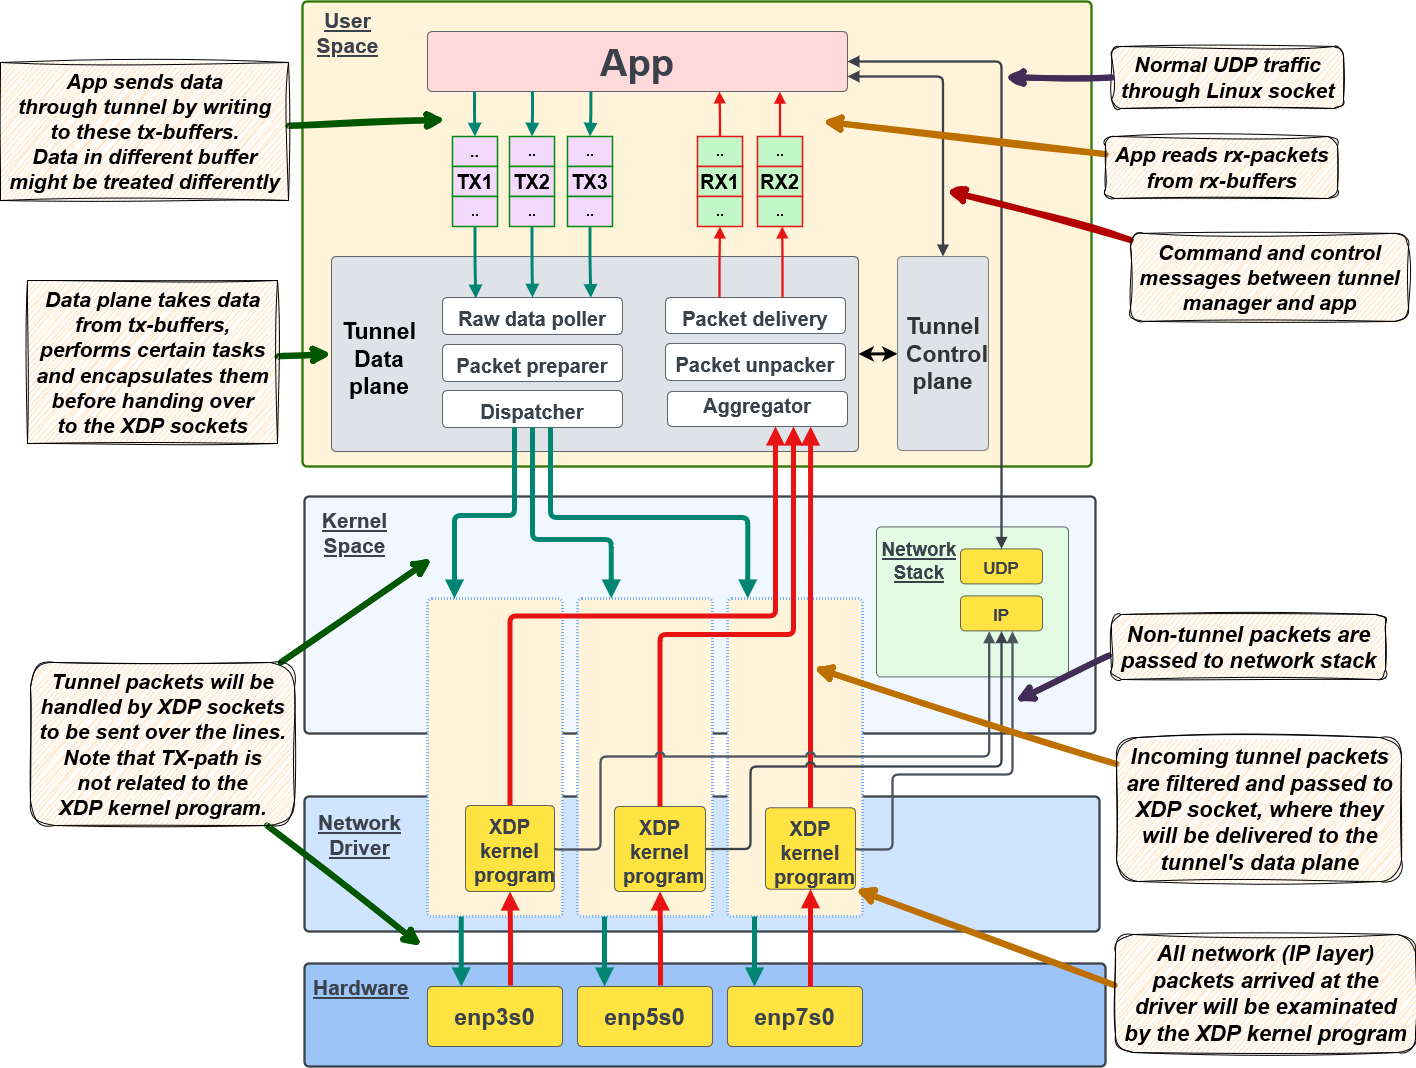
\includegraphics[width=1.0\textwidth]{mtx_design_and_workflow.png}
	\caption{The architecture of our MTX tunnel and the flow of packets. The notation \textit{1, 2 and 3} describe how  packets from application travel through the egress path. Notation \textit{4 to 8} show how application receive the packets from tunnel and normal Linux socket.}
	\label{fig:approach_design:mtx_design_and_workflow}
\end{figure}

The tunnel will be implemented in C for Linux. It consisted of 4 main components: eBPF kernel program, shared buffer, data plane and control plane.

\subsection{Buffers}
Buffers are separated into tx (transmit, see notation \textit{1}) and rx (receive, see notation \textit{8}) buffers that are available for application use. 
These buffers facilitate efficient data transfer for different streams and priorities, allowing the application to write to or read from the appropriate buffer as needed.

\subsection{Kernel Program}
XDP kernel program (see notation \textit{4}) is responsible for filtering tunnel packets based on criteria like UDP port, IP address, and the magic number in the tunnel header. 
These filtered packets are then delivered to the Packet aggregator for subsequent processing (notation \textit{5}). 
Conversely, all other packets that are not of interest to us are passed through to the Linux network stack (notation \textit{6 and 9}).
While it may be tempting to offload additional tasks such as unpacking and decryption to the kernel program for improved performance, it is important to note that this approach would significantly increase development time.

\subsection{Data Plane}
Data plane functionality is divided into two main paths: the TX path and the RX path.
\begin{itemize}
	\item TX path is responsible for data output and tunnel packet transmission. It consists of a poller that retrieves fresh packet data from the TX buffers, taking into account priorities for efficient processing. The poller determines the order in which packets are polled, considering factors such as smaller batch sizes and shorter timeouts to minimize waiting time and increase CPU usage. High-priority packets are processed first. After polling, the packet preparer handles tasks such as encryption, compression, and encapsulation. Finally, the dispatcher sends the prepared packets to the XDP sockets, which will then transmit them over the appropriate network links.
	\item RX path is responsible for receiving tunnel packets. The aggregator retrieves tunnel packets from the XDP sockets, and then passes them to the unpacker for unpacking and subsequent delivery to the RX buffers for further processing.
\end{itemize}

\subsection{Control Plane}
The control plane plays a vital role in the system as it handles various interactions with the application (notation \textit{7}). 
It is responsible for configuration management, initiation, termination, and runtime information exchange. 
The control plane acts as the central control hub, governing and coordinating all other components of the tunnel.


\section{Characteristics of MTX}
At the conclusion of our project, we aim to provide an MTX library equipped with a comprehensive range of features, including:

\begin{itemize}
	\item Embrace a contemporary approach to system and network programming with the utilization of eBPF technology, ensuring performance, safety, and freedom from legacy code.
	\item Highly likely to outperform alternative user-space approaches significantly.
	\item Enhance redundancy and bolster connection reliability.
	\item Potential for improved latency by leveraging efficiency and harnessing the power of multipath.
	\item Address the varying requirements of different stream types by optimizing line utilization: bandwidth for data-intensive tasks, low latency for voice-over-IP, and reliable transmission for critical messages.
\end{itemize}

The MTX tunnel incorporates a flexible policy framework at multiple layers, enabling the utilization of algorithms or configurations. 
This offers a wide array of options for customization, including at:
\begin{itemize}
	\item Data link layer: determining which streams can utilize specific links, assigning priorities, and implementing load distribution policies.
	\item Network layer: selecting the carrier protocol (IPv4/v6) and specifying the UDP port.
	\item Application layer: prioritizing applications, defining buffer fetching timeouts, reserving buffers for low-latency usage, and more.
\end{itemize}

Ideally, a tunnel control plane will operate in the background after initiation, effectively managing the streams utilized by various applications. 
These applications will register their usage with the tunnel control plane and interact with the data plane through shared buffers. 
Parameters can be individually configured for each application.
Additionally, we will explore the feasibility of creating a TUN/TAP interface to serve as an intermediate communication layer between the MTX tunnel and applications. 
This approach, commonly employed by VPN programs, enables multiple applications to utilize the tunnel connection without requiring modifications to their source code.
